\documentclass[a4paper,12pt]{article}
\usepackage[utf8]{inputenc} % Encodage des caractères
\usepackage[T1]{fontenc} % Encodage de la police
\usepackage{lipsum} % Pour générer du texte factice
\usepackage{graphicx} % Pour inclure des images
\usepackage{amsmath} % Pour les équations mathématiques
\usepackage{amssymb} % Pour les symboles mathématiques
\usepackage[hidelinks]{hyperref} % Pour les hyperliens
\usepackage{float} % À ajouter dans le préambule pour utiliser l'option H

\title{Bio Ingénierie \\
	ENISE Génie Sensoriel - S9}
\author{Maxime BEL}

\begin{document}
	
\maketitle
% Insertion de la table des matières
\tableofcontents
\clearpage


\clearpage
\section{Étude des Contraintes}


\subsection{Un paramètre important : le rayon}





\begin{abstract}
Le but est d'analyser le contact entre une sphère (E = 210GPa) de différents rayon (10mm, 5mm, 2mm, 0.5mm) à une force donnée (50N) contre une surface polymère plane (E = 10MPa) et dans un autre cas, contre une surface sphèrique, une sphère de même rayon (E = 210GPa).\\
Cette analyse sert à comprendre de quelle manière les matériaux se déforment et comment les contraintes intérieures et extérieures se répartissent au niveau de la zone de contact ainsi qu'en profondeur.\\
\end{abstract}

\begin{center}
	\textbf{Matériels \& Méthodes}
\end{center}

Nous utiliserons des systèmes de coordonnées polaires car nous étudions une sphère. On notera les contraintes radiales $\sigma_{r}$, les contraintes angulaires $\sigma_{\theta}$ et les contraintes axiales $\sigma_{z}$.\\
Nous étudierons 2 à 2 les contactes sphère-sphère et sphère-polymère pour chaque types de contraintes.
\bigskip
\\
Nous utiliserons les formules adéquates :\\
On met en relation les 2 modules de Young notés $E_1$ et $E_2$ pour les 2 coefficients de poisson notés $\nu_1$ et $\nu_2$.\eqref{eq:1}\\
\begin{equation}
	\frac{1}{E^*} = \frac{1 - \nu_1^2}{E_1} + \frac{1 - \nu_2^2}{E_2}
	\label{eq:1}
\end{equation}

Le rayon équivalent est utilisée de la même manière pour mettre en relation les 2 surfaces de contact. Lorsque c'est un contact sphère-plan, alors le rayon du plan est infini et le rayon pris en compte est celui de la sphère. Lorsque c'est un contact sphère-sphère, alors, nous utilisons la formule ci-dessus.\eqref{eq:2}\\
\begin{equation}
	R^* = \frac{1}{R_1} + \frac{1}{R_2}
	\label{eq:2}
\end{equation}
Le rayon de contact noté a est le rayon de la surface créé lorsque les 2 surfaces se rencontrent.\eqref{eq:3}
\begin{equation}
	a = \left(\frac{3 F R^*}{4 E^*}\right)^{\frac{1}{3}}
	\label{eq:3}
\end{equation}

\clearpage
La pression maximale exercée au centre du cercle de contact notée $p_0$.\eqref{eq:4}\\
\begin{equation}
	p_0 = \frac{3 F}{2 \pi a^2}
	\label{eq:4}
\end{equation}
Nous afficherons sur la même courbe du graphique les contraintes radiales intérieures et extérieures car elles sont complémentaires, nous pourrons les visualiser séparément en se repérant grâce à l'abscisse représentant le rayon de contact.\eqref{eq:5}\eqref{eq:6}
\begin{equation}
	\frac{\sigma_{r\_int}}{p_0} = \left( \frac{1 - 2 \nu}{3} \cdot \frac{a^2}{r^2} \left(1 - \left(1 - \frac{r^2}{a^2}\right)^{\frac{3}{2}}\right) - \sqrt{1 - \frac{r^2}{a^2}} \right)
	\label{eq:5}
\end{equation}
\begin{equation}
	\frac{\sigma_{r\_ext}}{p_0} = \frac{(1 - 2 \nu) \cdot a^2}{3 r^2}
	\label{eq:6}
\end{equation}
De la même manière pour les contraintes angulaires intérieures et extérieures.\eqref{eq:7}\eqref{eq:8}
\begin{equation}
	\frac{\sigma_{\theta\_int}}{p_0} = \left( -\frac{1 - 2 \nu}{3} \cdot \frac{a^2}{r^2} \left(1 - \left(1 - \frac{r^2}{a^2}\right)^{\frac{3}{2}}\right) - 2 \nu \sqrt{1 - \frac{r^2}{a^2}} \right)
	\label{eq:7}
\end{equation}
\begin{equation}
	\frac{\sigma_{\theta\_ext}}{p_0} = - \frac{(1 - 2 \nu) \cdot a^2}{3 r^2}
	\label{eq:8}
\end{equation}
Finalement, la contrainte axiale. \eqref{eq:9}
\begin{equation}
	\frac{\sigma_{z}}{p_0} = - \sqrt{1 - \left(\frac{r}{a}\right)^2}
	\label{eq:9}
\end{equation}


\begin{center}
	\textbf{Résultats}
\end{center}
Étudions alors les contraintes radiales sur un contact sphère-sphère et sphère-polymère(plan).
\bigskip
\\
On peut remarquer une courbe symétrique par rapport à l'axe des ordonnées, ce qui est assez intuitif avec un contact sphère supposée parfaitement ronde.\\
De plus, on remarque que pour une force donnée, le rayon est un facteur qui agit sur la contrainte : plus le rayon est grand et plus les contraintes intérieures et extérieures en valeur absolue diminuent.\hyperref[fig:mon_image1]{Fig(1)}
\begin{figure}[H] % Position de l'image : ici [h] pour "ici" (here)
	\centering
	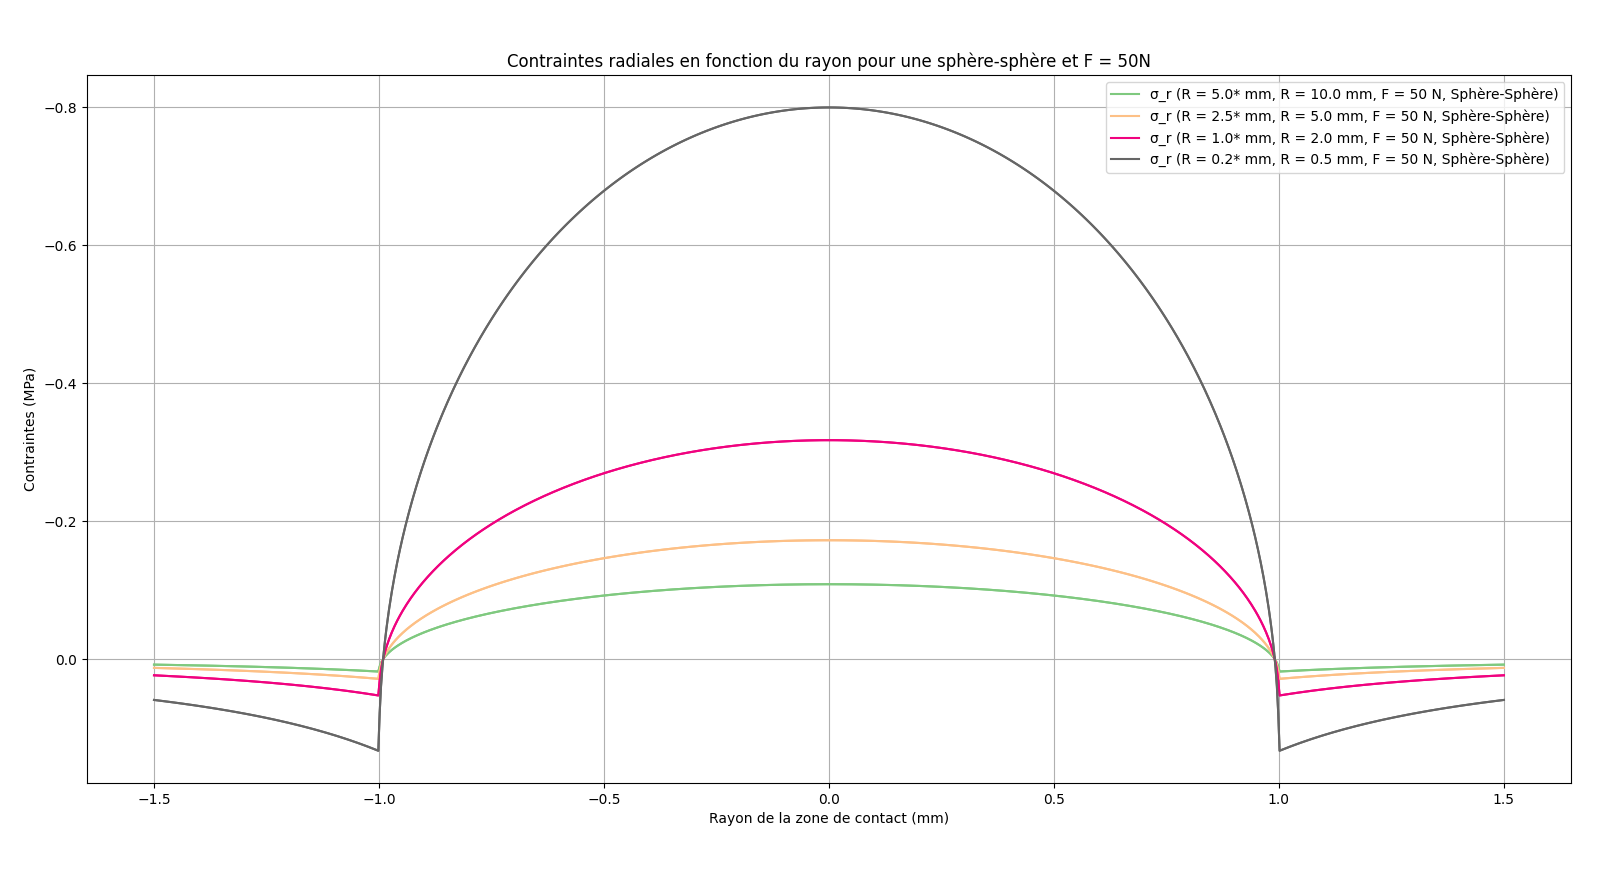
\includegraphics[width=0.9\textwidth]{rad1.png} % Ajuste la largeur de l'image
	\caption{Contraintes radiales en fonction du rayon pour une sphère-sphère et F = 50N} % Texte de la légende
	\label{fig:mon_image1} % Label pour faire référence à l'image dans le texte
\end{figure}
On remarque sur \hyperref[fig:mon_image2]{Fig(2)} que le module d'Young et donc le coefficient de poisson de la surface en contact avec la sphère agit sur les contraintes radiales.
\begin{figure}[H] % Position de l'image : ici [h] pour "ici" (here)
	\centering
	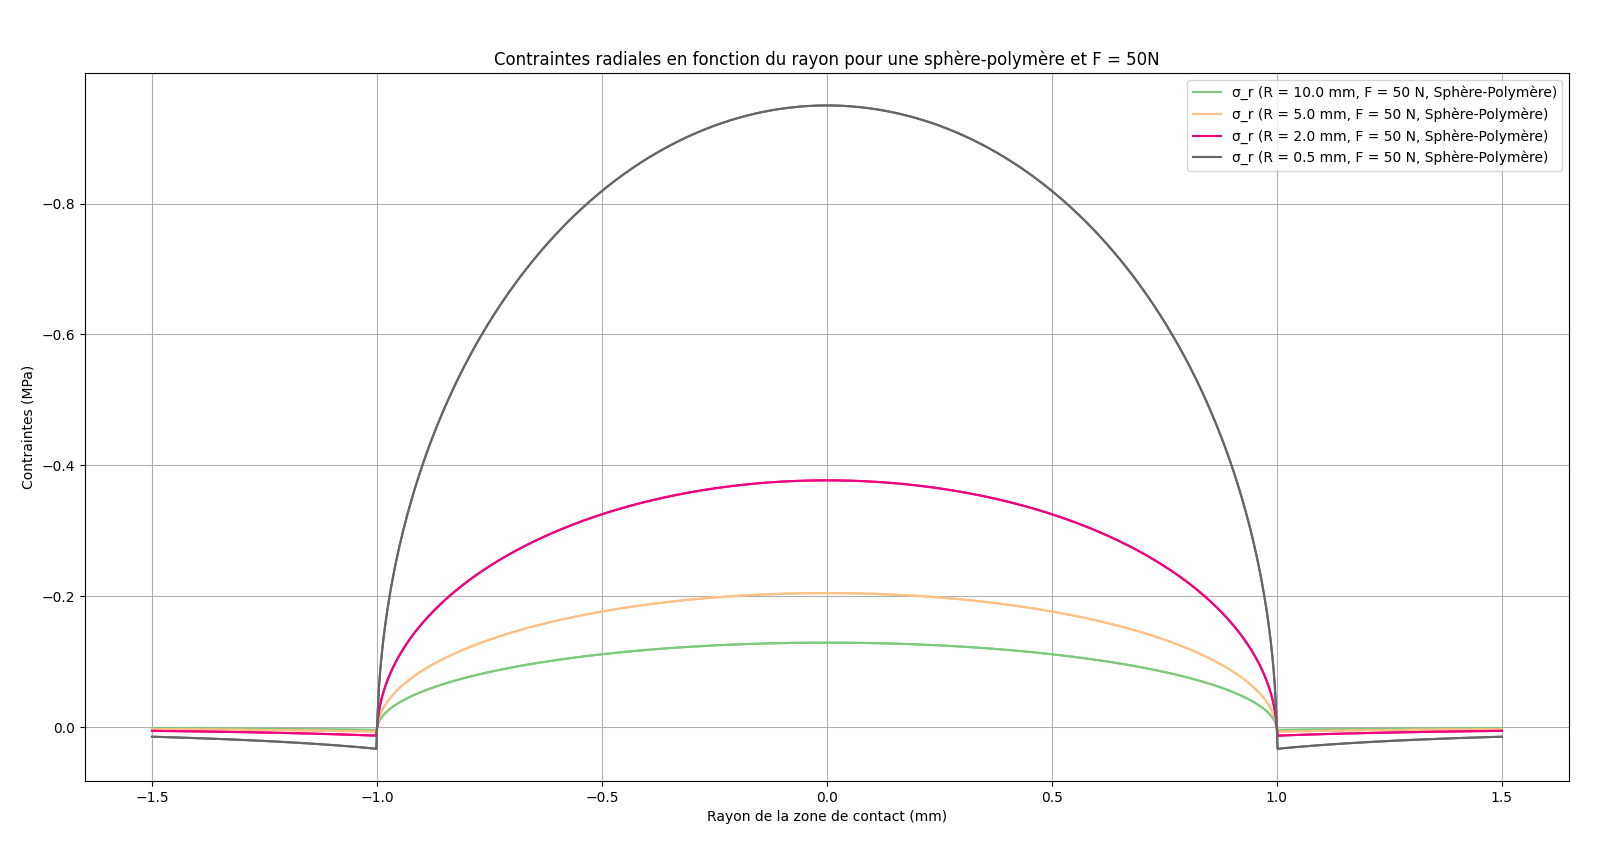
\includegraphics[width=1\textwidth]{rad2.png} % Ajuste la largeur de l'image
	\caption{Contraintes radiales en fonction du rayon pour une sphère-polymère et F = 50N} % Texte de la légende
	\label{fig:mon_image2} % Label pour faire référence à l'image dans le texte
\end{figure}
\clearpage
De la même manière, on peut regarder la contrainte axiale qui elle aussi est une courbe symmétrique par rapport à l'axe des ordonnées et qui diminue lorsque le rayon augmente également.\hyperref[fig:mon_image3]{Fig(3)}
\begin{figure}[H] % Position de l'image : ici [h] pour "ici" (here)
	\centering
	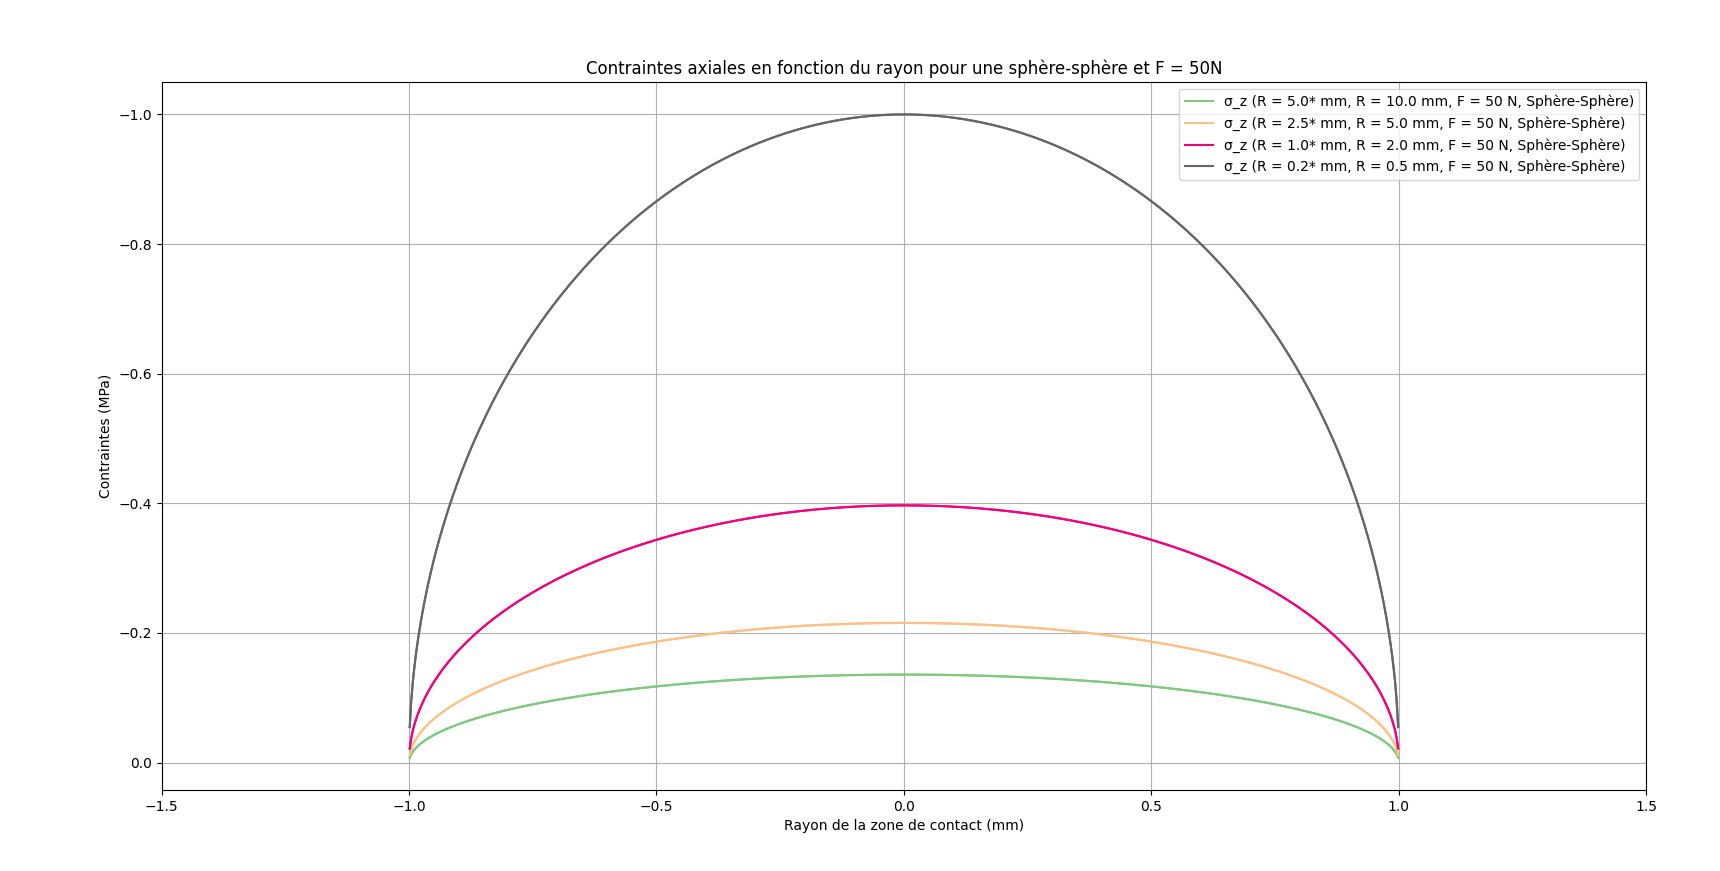
\includegraphics[width=0.9\textwidth]{ax1.png} % Ajuste la largeur de l'image
	\caption{Contraintes axiales en fonction du rayon pour une sphère-sphère et F = 50N} % Texte de la légende
	\label{fig:mon_image3} % Label pour faire référence à l'image dans le texte
\end{figure}
Or, la surface de contact à la sphère n'agit pas sur la contrainte axiale comme nous le montre la \hyperref[fig:mon_image4]{Fig(4)}
\begin{figure}[H] % Position de l'image : ici [h] pour "ici" (here)
	\centering
	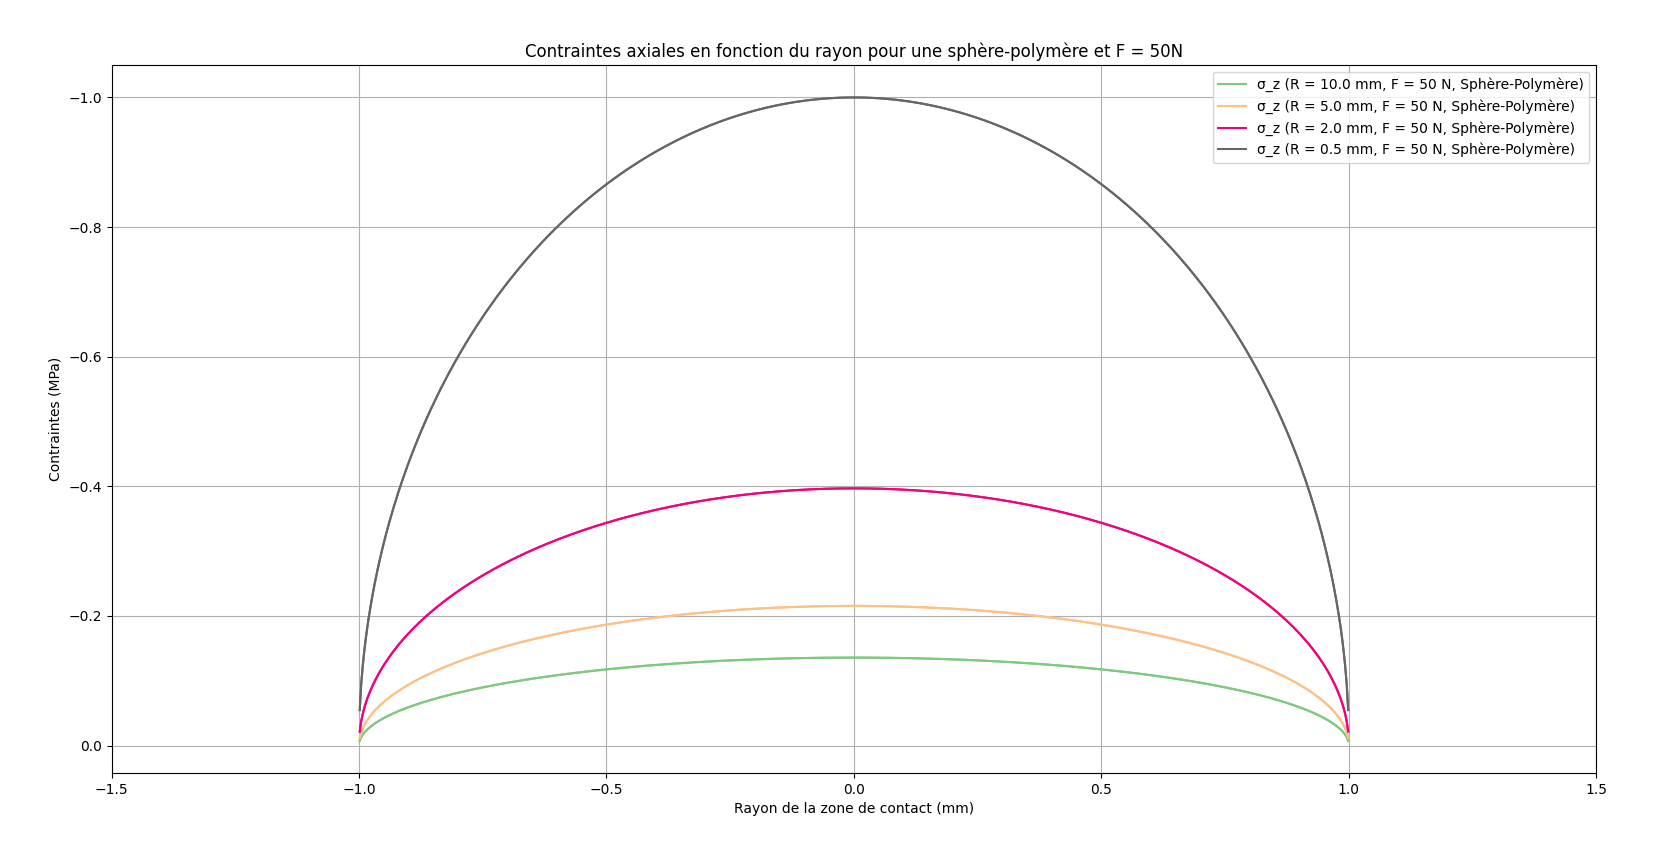
\includegraphics[width=0.9\textwidth]{ax2.png} % Ajuste la largeur de l'image
	\caption{Contraintes axiales en fonction du rayon pour une sphère-polymère et F = 50N} % Texte de la légende
	\label{fig:mon_image4} % Label pour faire référence à l'image dans le texte
\end{figure}
\clearpage
On remarque toujours la symétrie par rapport à l'axe des ordonnées. De plus, les contraintes intérieures angulaires et radiales présentent des similitudes, la principale différence étant que la contrainte intérieure angulaire, la plus éloignée du centre du cercle de contact, est négative, tandis que la contrainte intérieure radiale à la même distance est positive. Ainsi, à mesure que l'on s'éloigne du centre du cercle de contact, les contraintes diminuent, indépendamment de la direction. \hyperref[fig:mon_image5]{Fig(5)}
\begin{figure}[H] % Position de l'image : ici [h] pour "ici" (here)
	\centering
	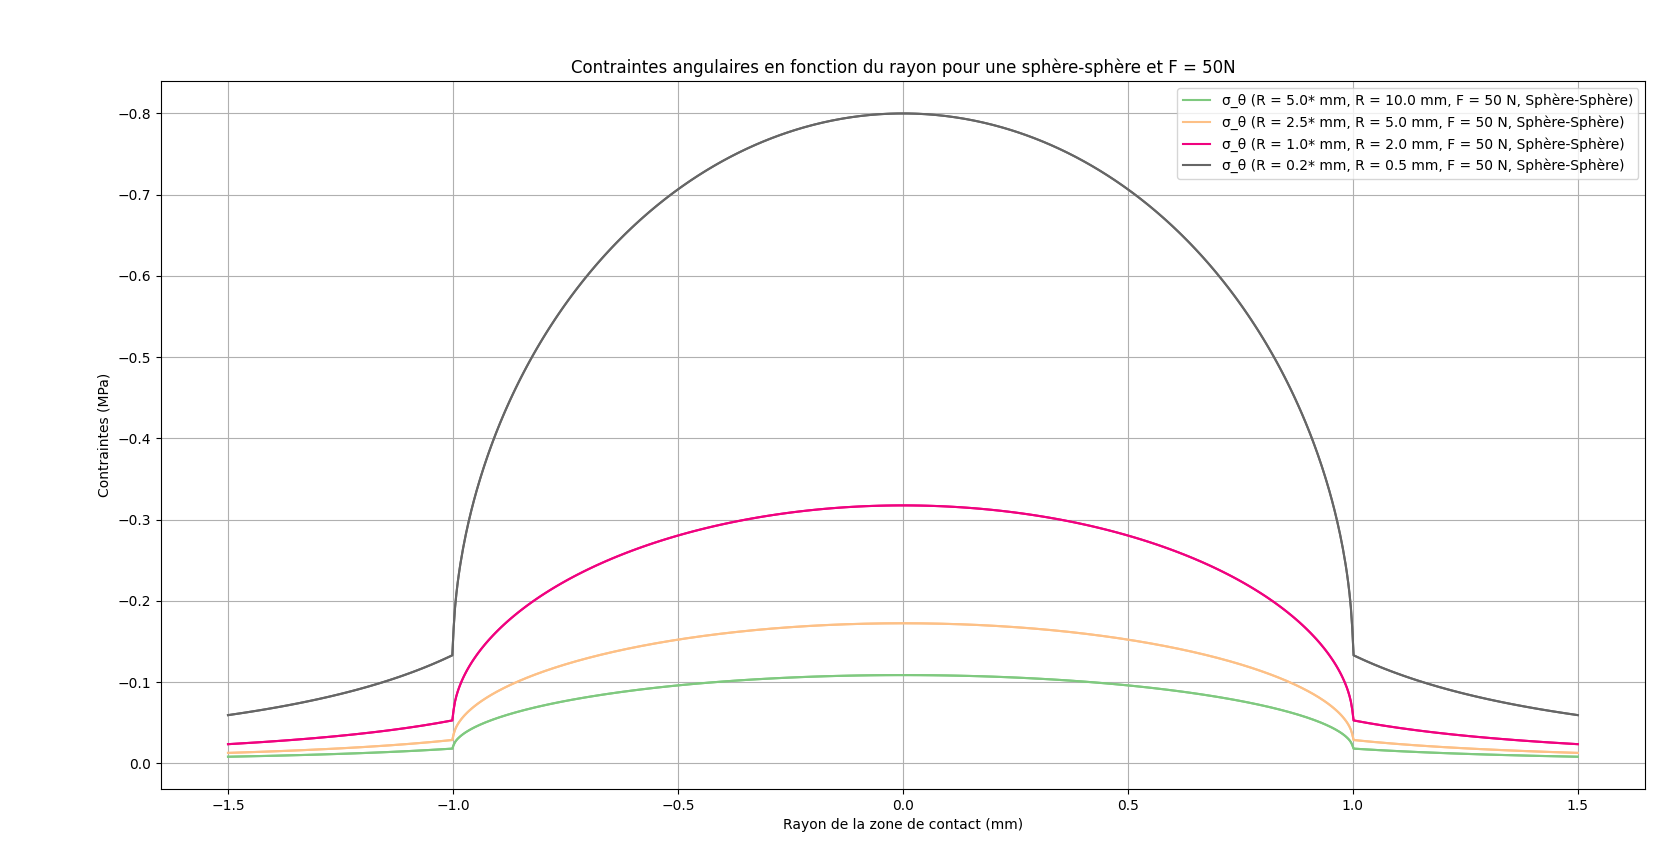
\includegraphics[width=0.8\textwidth]{ang1.png} % Ajuste la largeur de l'image
	\caption{Contraintes angulaires en fonction du rayon pour une sphère-polymère et F = 50N} % Texte de la légende
	\label{fig:mon_image5} % Label pour faire référence à l'image dans le texte
\end{figure}
On remarque que la même logique précédemment s'applique sur tout type de contact.\hyperref[fig:mon_image6]{Fig(6)}
\begin{figure}[H] % Position de l'image : ici [h] pour "ici" (here)
	\centering
	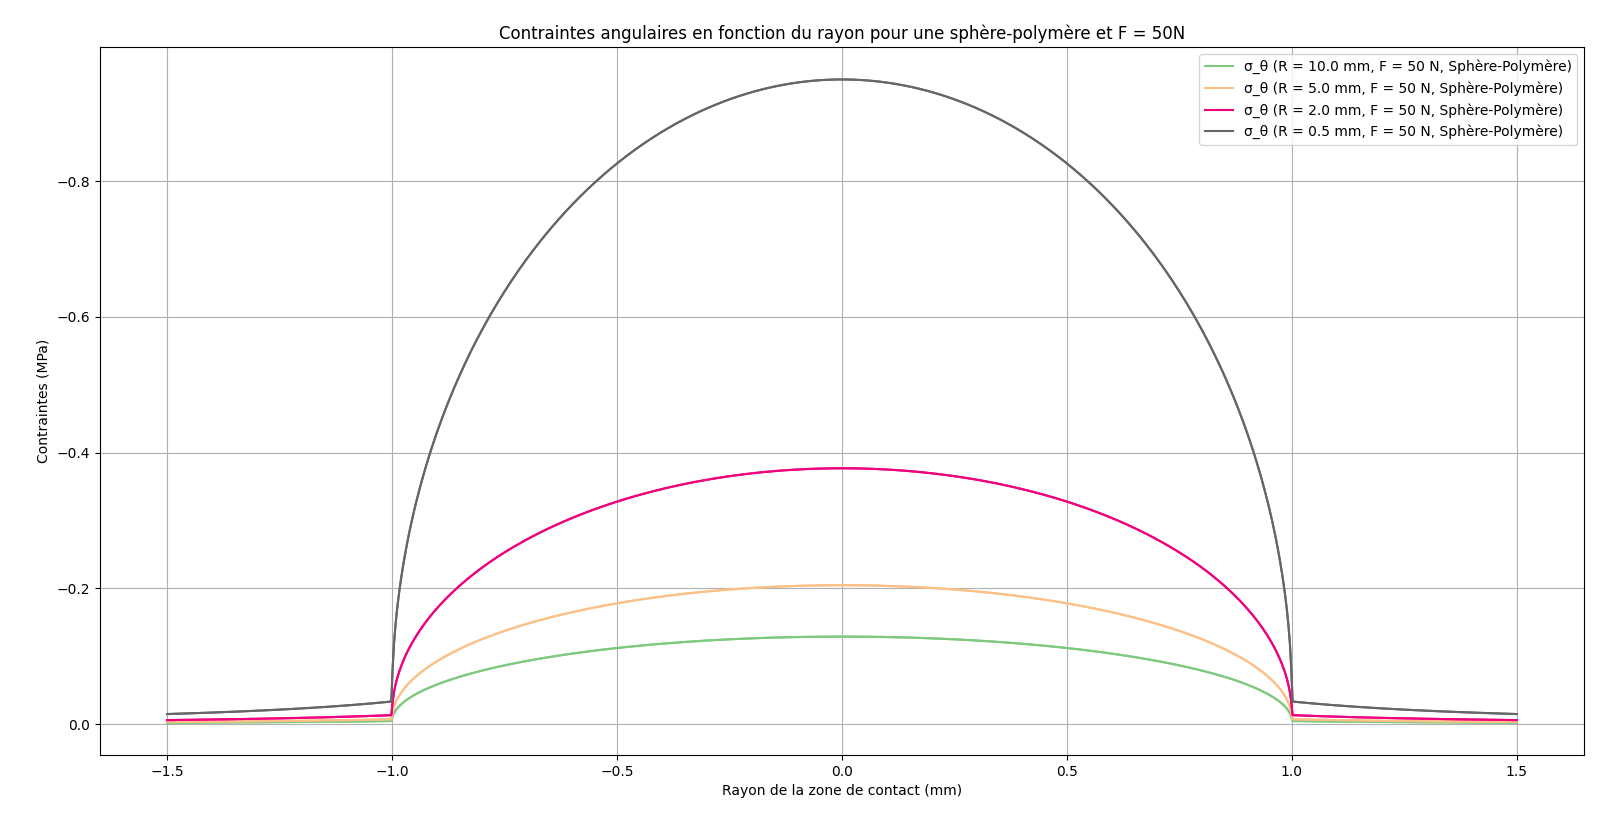
\includegraphics[width=0.8\textwidth]{ang2.png} % Ajuste la largeur de l'image
	\caption{Contraintes angulaires en fonction du rayon pour une sphère-polymère et F = 50N} % Texte de la légende
	\label{fig:mon_image6} % Label pour faire référence à l'image dans le texte
\end{figure}
\clearpage


\subsection{Un paramètre important : la force}
Par analogie, nous présenterons les mêmes graphiques mais cette fois-ci en fixant le rayon et en changeant la force exercée (50N et 100N).
\begin{figure}[H] % Position de l'image : ici [h] pour "ici" (here)
	\centering
	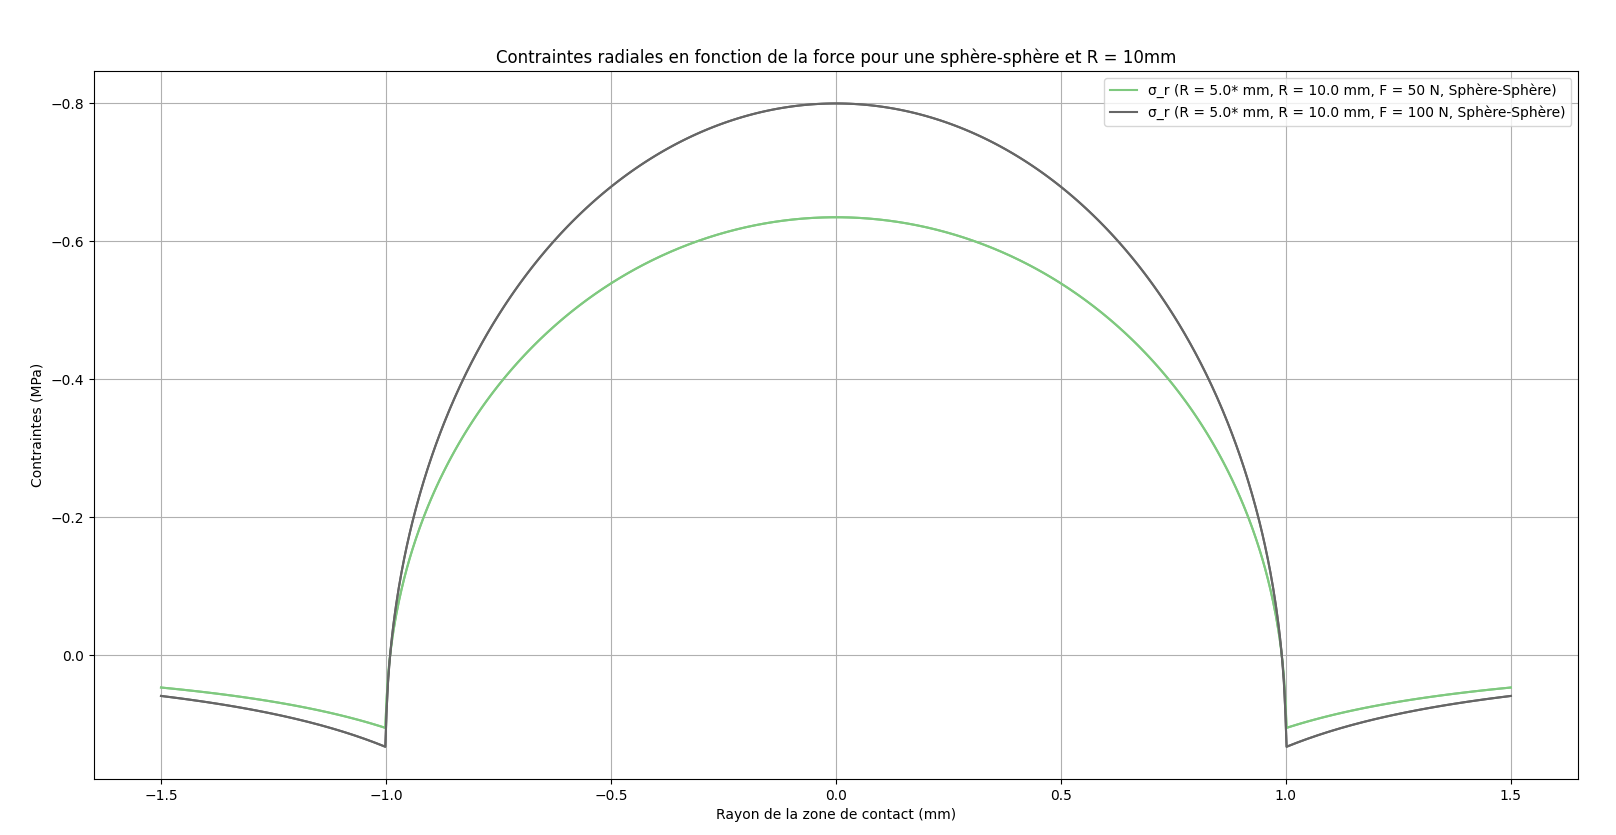
\includegraphics[width=0.9\textwidth]{rad3.png} % Ajuste la largeur de l'image
	\caption{Contraintes radiales en fonction de la force pour une sphère-sphère et R = 10mm} % Texte de la légende
	\label{fig:mon_image7} % Label pour faire référence à l'image dans le texte
\end{figure}

\begin{figure}[H] % Position de l'image : ici [h] pour "ici" (here)
	\centering
	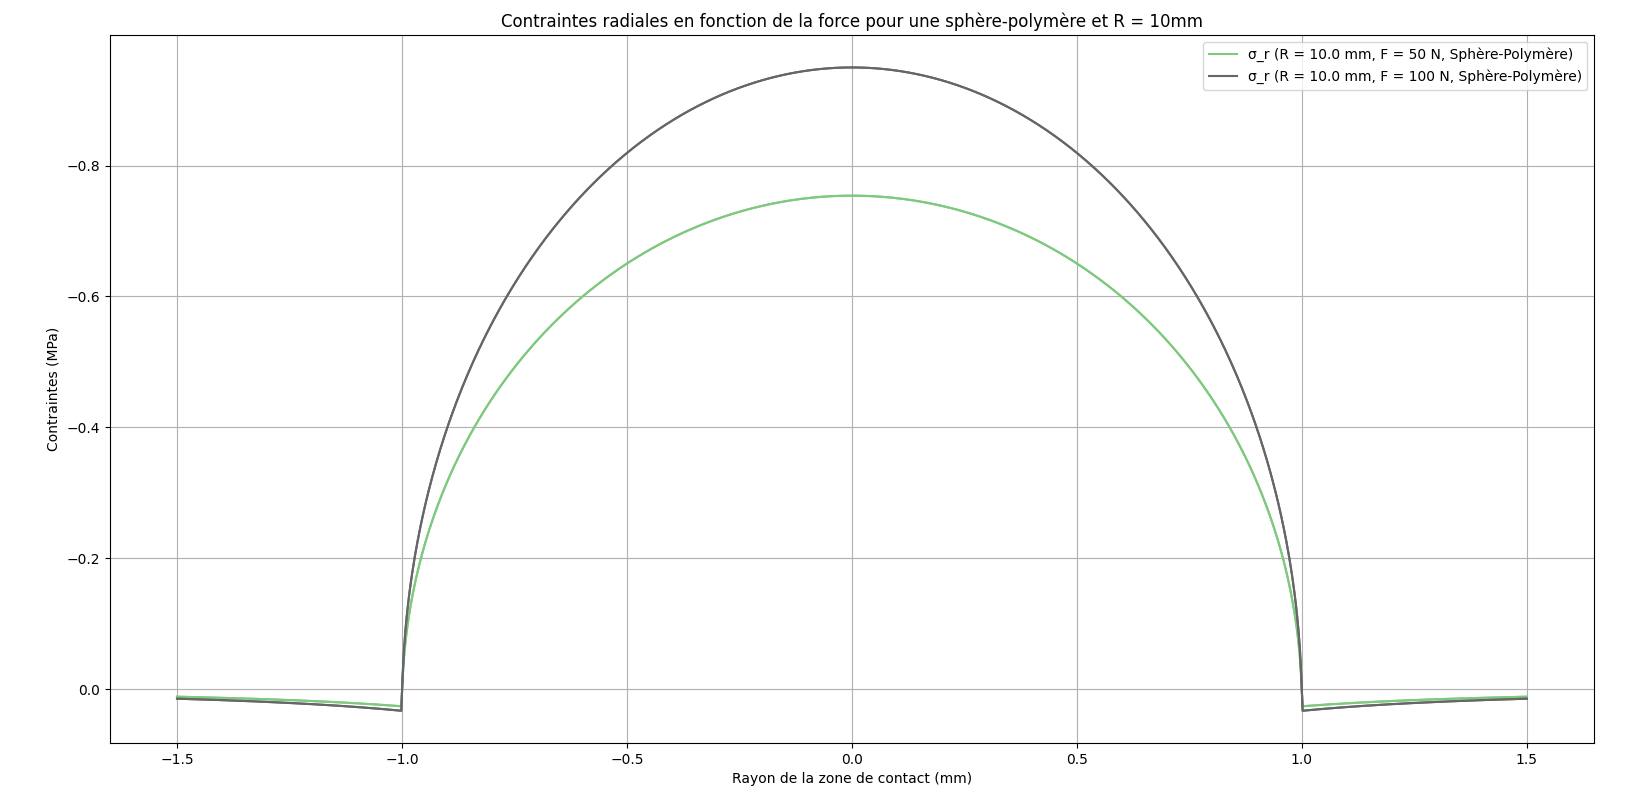
\includegraphics[width=0.9\textwidth]{rad4.png} % Ajuste la largeur de l'image
	\caption{Contraintes radiales en fonction de la force pour une sphère-polymère et R = 10mm} % Texte de la légende
	\label{fig:mon_image8} % Label pour faire référence à l'image dans le texte
\end{figure}
\clearpage
\begin{figure}[H] % Position de l'image : ici [h] pour "ici" (here)
	\centering
	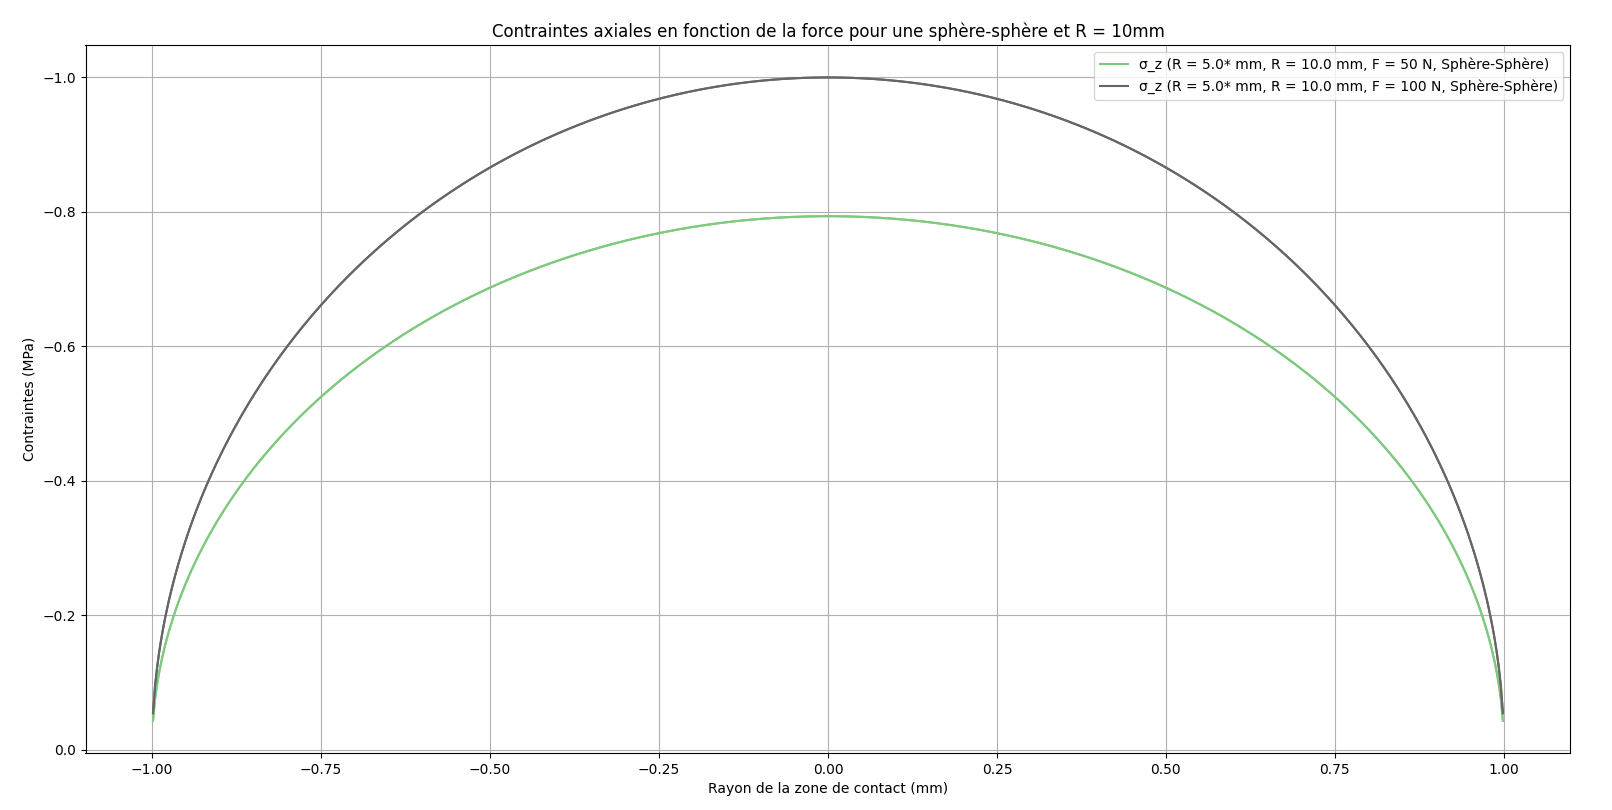
\includegraphics[width=0.9\textwidth]{ax3.png} % Ajuste la largeur de l'image
	\caption{Contraintes axiales en fonction de la force pour une sphère-sphère et R = 10mm} % Texte de la légende
	\label{fig:mon_image9} % Label pour faire référence à l'image dans le texte
\end{figure}

\begin{figure}[H] % Position de l'image : ici [h] pour "ici" (here)
	\centering
	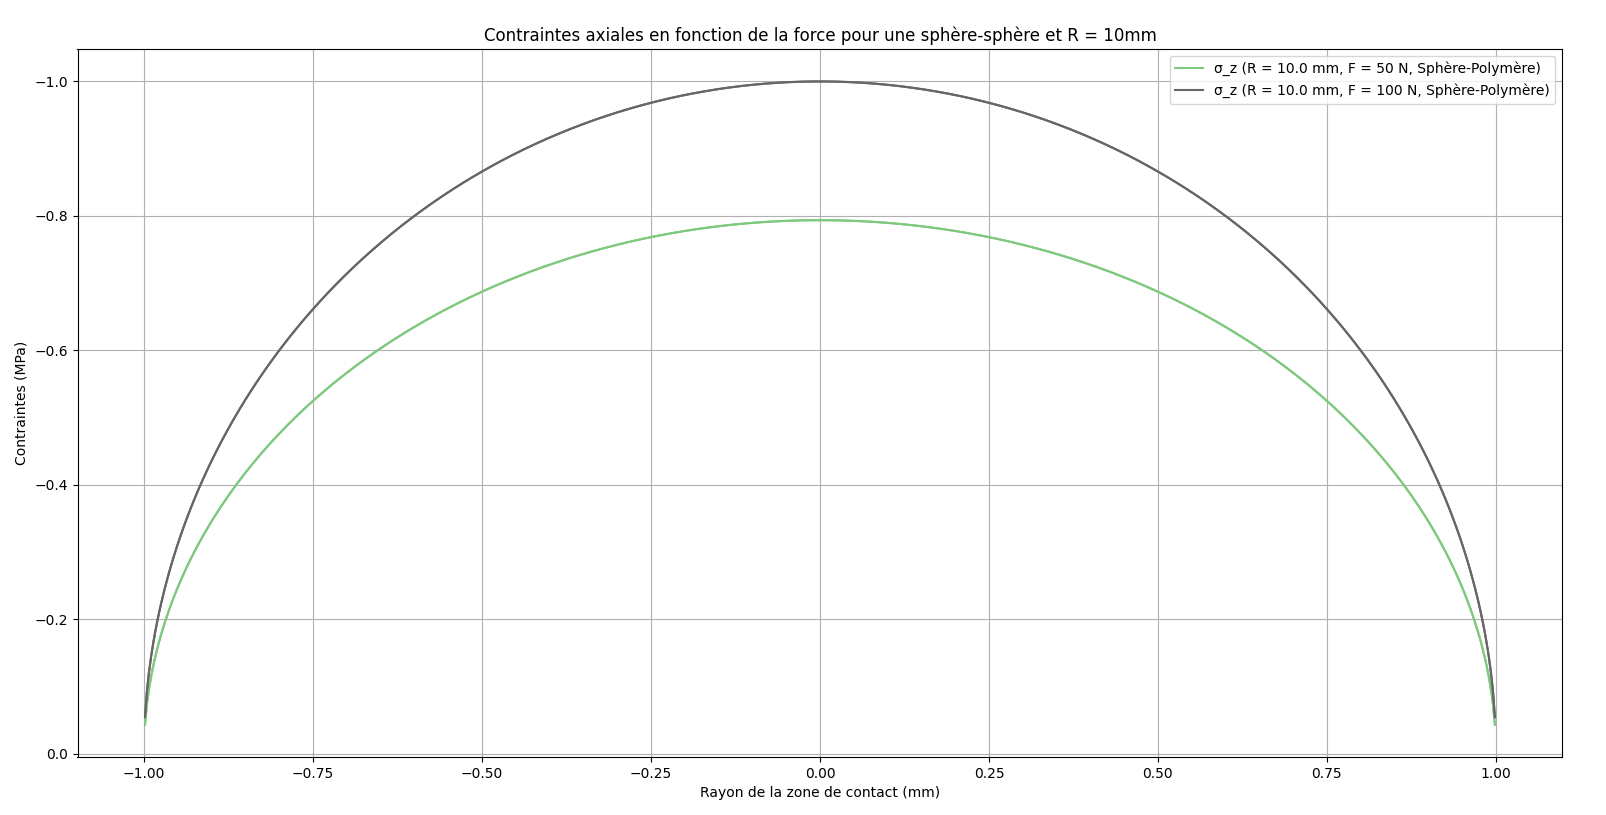
\includegraphics[width=0.9\textwidth]{ax4.png} % Ajuste la largeur de l'image
	\caption{Contraintes axiales en fonction de la force pour une sphère-polymère et R = 10mm} % Texte de la légende
	\label{fig:mon_image10} % Label pour faire référence à l'image dans le texte
\end{figure}
\clearpage
\begin{figure}[H] % Position de l'image : ici [h] pour "ici" (here)
	\centering
	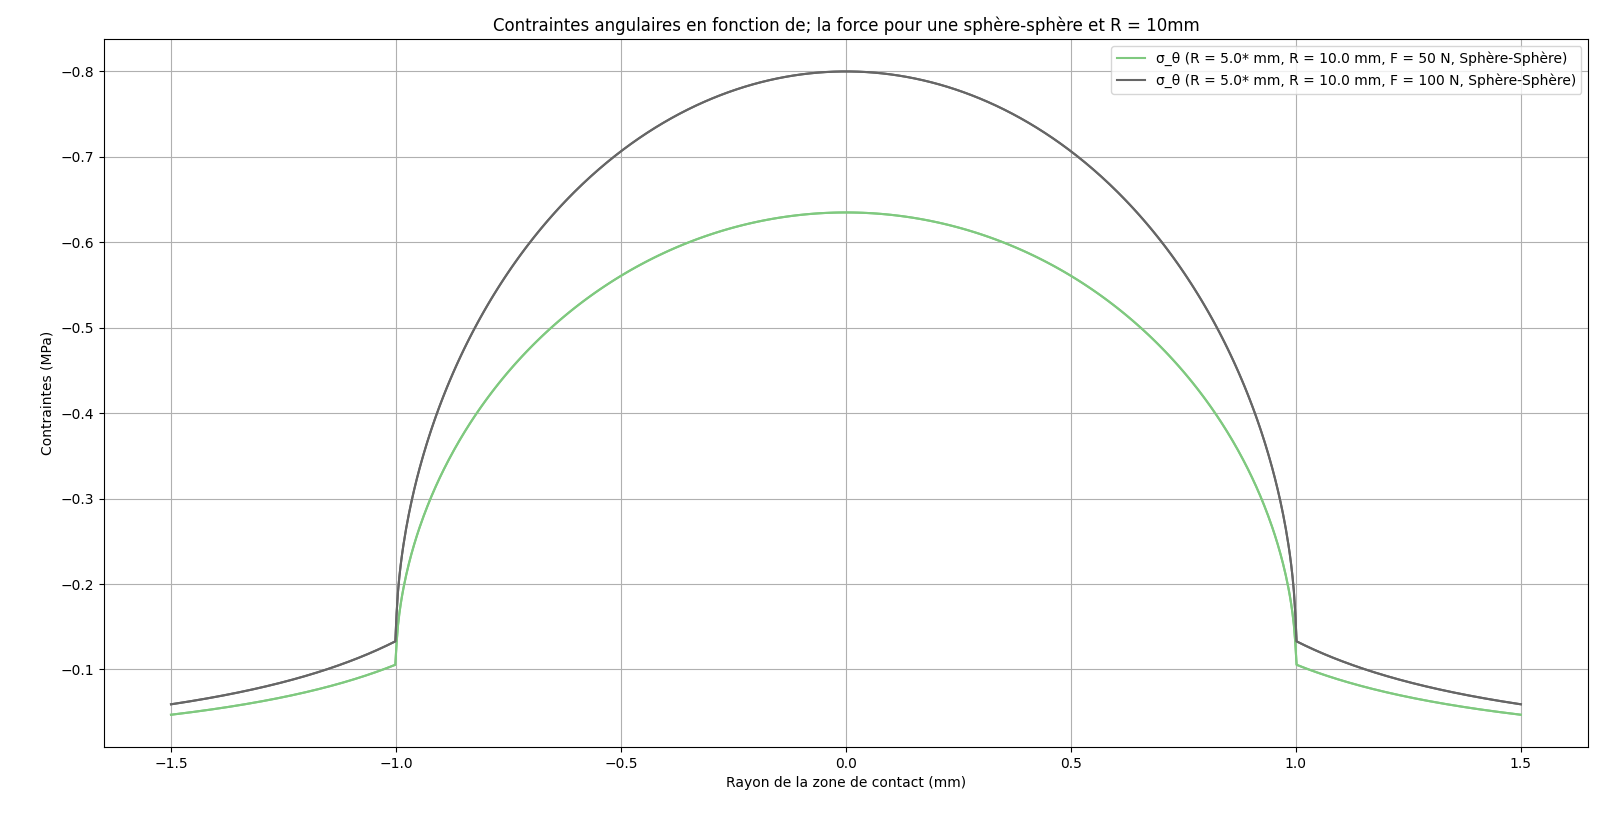
\includegraphics[width=0.9\textwidth]{ang3.png} % Ajuste la largeur de l'image
	\caption{Contraintes angulaires en fonction de la force pour une sphère-sphère et R = 10mm} % Texte de la légende
	\label{fig:mon_image11} % Label pour faire référence à l'image dans le texte
\end{figure}

\begin{figure}[H] % Position de l'image : ici [h] pour "ici" (here)
	\centering
	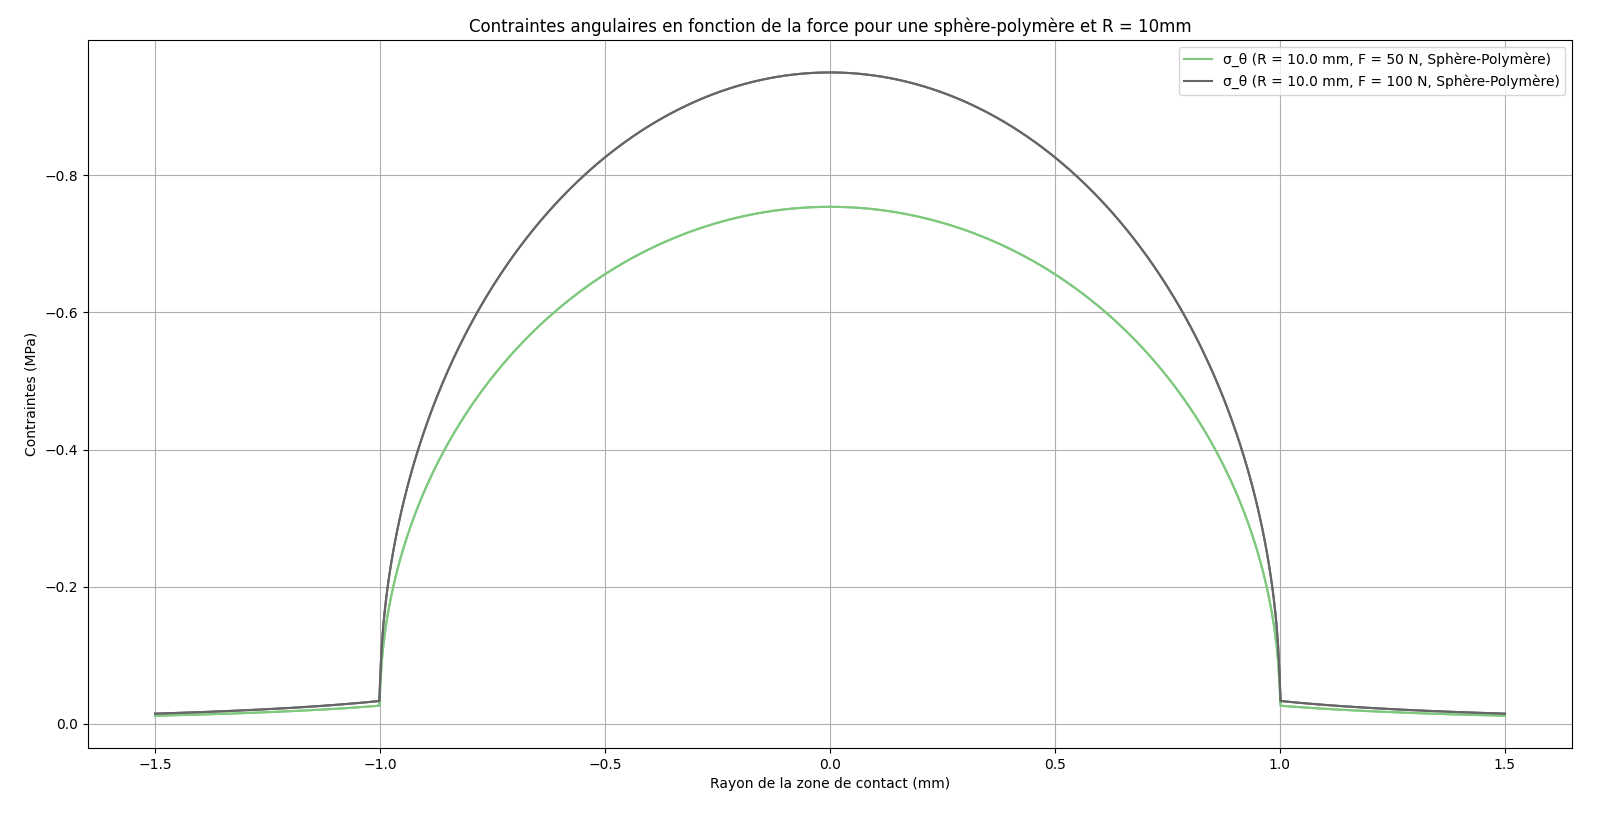
\includegraphics[width=0.9\textwidth]{ang4.png} % Ajuste la largeur de l'image
	\caption{Contraintes angulaires en fonction de la force pour une sphère-polymère et R = 10mm} % Texte de la légende
	\label{fig:mon_image12} % Label pour faire référence à l'image dans le texte
\end{figure}
\clearpage
\section{Biopsie}


\section{Pression de contact}

\end{document}
